\chapter{Numerical results}

Since we don't have the exact solution, we have implemented the implicit Euler method given in paper '\textit{A robust and accurate finite difference method for a generalized Black-Scholes equation}' (which the author have also used) and we take this as exact solution with N = 1024 and M = 1024, since we know this method converges. Because we only know ”the exact solution” on mesh points, we use the linear interpolation to get solutions at other points. The file 'exact\_robust.m' contains the implementation of implicit Euler method used as exact solution. Exponential time integration and second order difference scheme is implemented with \textbf{'Exp\_1.m'} and \textbf{'Exp\_2.m'} files.

The file 'Exp\_1.m' plots European option price with parameters $\sigma = 0.2 + 0.2(1 - t)((x/25-1.2)^2/((x/25)^2 + 1.44))$, r = 0.06, T = 1, K = 25 and $S_{max} = 100$ and calculates error and convergence rate. Output of the program is given in fig \ref{fig1} and table \ref{table1}.

\begin{figure}[h]
\centering
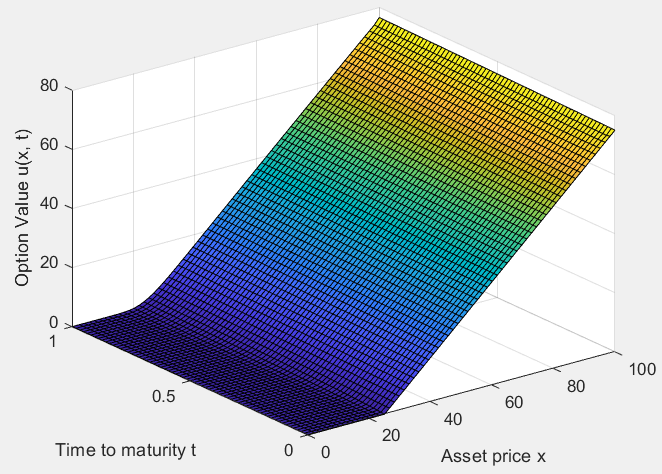
\includegraphics[width=1\textwidth]{figures/fig1.PNG}
\caption{Computed option value for Test 1}
\label{fig1}
\end{figure}

\bgroup
\def\arraystretch{1.5}
\begin{table}[H]
    \caption{Numerical results for Test 1}    % title of Table
    \label{table1}
    \vspace{1mm}
    \centering                              % used for centering table
    \begin{tabular}{c c c c c c}              % centered columns (6 columns)
    \hline\hline                            % inserts double horizontal lines
    M & N & Exp Error & Exp Rate & Implicit Error & Implicit rate \\ [0.5ex] 
    % inserts table heading
    \hline                              % inserts single horizontal line
    16 & 64 & 0.37941 & 2.3351 & 0.14668 & 1.0995 \\
    32 & 128 & 0.032271 & 1.2515 & 0.068448 & 1.2224 \\
    64 & 256 & 0.02959 & -- & 0.029335 & -- \\ [1ex]         % [1ex] adds vertical space
    \hline                              % inserts single line
    \end{tabular}
    \label{table:nonlin}                % is used to refer this table in the text
\end{table}
\egroup



The file \textbf{'Exp\_2.m'} plots the European option price with parameters $\sigma = 0.2(1 + (0.1(1 - t))(x/(1+x)))$, r = 0.06, T = 1, K = 25 and $S_{max} = 100$ and also calculates the error and convergence rate. Output of the program is given in fig \ref{fig2} and table \ref{table2}.

\begin{figure}[h]
\centering
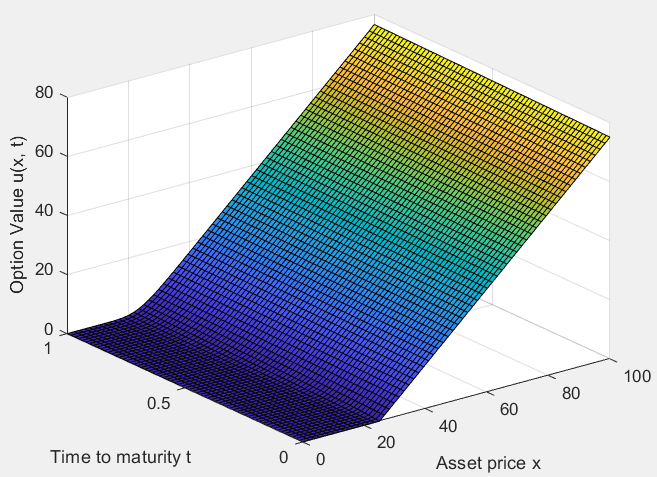
\includegraphics[width=1\textwidth]{figures/fig2.PNG}
\caption{Computed option value for Test 2}
\label{fig2}
\end{figure}

\bgroup
\def\arraystretch{1.5}
\begin{table}[H]
    \caption{Numerical results for Test 2}    % title of Table
    \label{table2}
    \vspace{1mm}
    \centering                              % used for centering table
    \begin{tabular}{c c c c c c}              % centered columns (6 columns)
    \hline\hline                            % inserts double horizontal lines
    M & N & Exp Error & Exp Rate & Implicit Error & Implicit rate \\ [0.5ex] 
    % inserts table heading
    \hline                              % inserts single horizontal line
    16 & 64 & 0.38644 & 2.2826 & 0.14668 & 1.0995 \\
    32 & 128 & 0.032989 & 1.2232 & 0.068448 & 1.2224 \\
    64 & 256 & 0.030307 & -- & 0.029335 & -- \\ [1ex]         % [1ex] adds vertical space
    \hline                              % inserts single line
    \end{tabular}
    \label{table:nonlin}                % is used to refer this table in the text
\end{table}
\egroup


By looking at the figures, it is evident that the numerical solutions by the method are non-oscillatory. Tables \ref{table1} and \ref{table2} show that the exponential time integration method converges more rapidly than the implicit Euler method. Nevertheless, exponential time integration method requires more computer time than implicit Euler method for the same M and N. Although it cannot be reached by large M and N, exponential time integration rate is close to 2 due to the fact that there is no actual "exact solution".